\documentclass{beamer}

\usepackage[frenchb]{babel}
\usepackage[T1]{fontenc}
\usepackage[utf8]{inputenc}

\usepackage{pgfplots}
\usepackage{pgfplotstable}
\usepackage{graphicx}
\pgfplotsset{compat=1.5}

\usepackage[squaren, Gray, cdot]{SIunits}

\usetheme{Warsaw}

\beamertemplatenavigationsymbolsempty 

\title{Paramétrage des lifters}
\author{Mathieu Bour}
\date{2016 - 2017}

\begin{document}
	\begin{frame}
		\titlepage
	\end{frame}

	\section{Préambule}
		\begin{frame}{Définition}
			\begin{figure}
				\center
				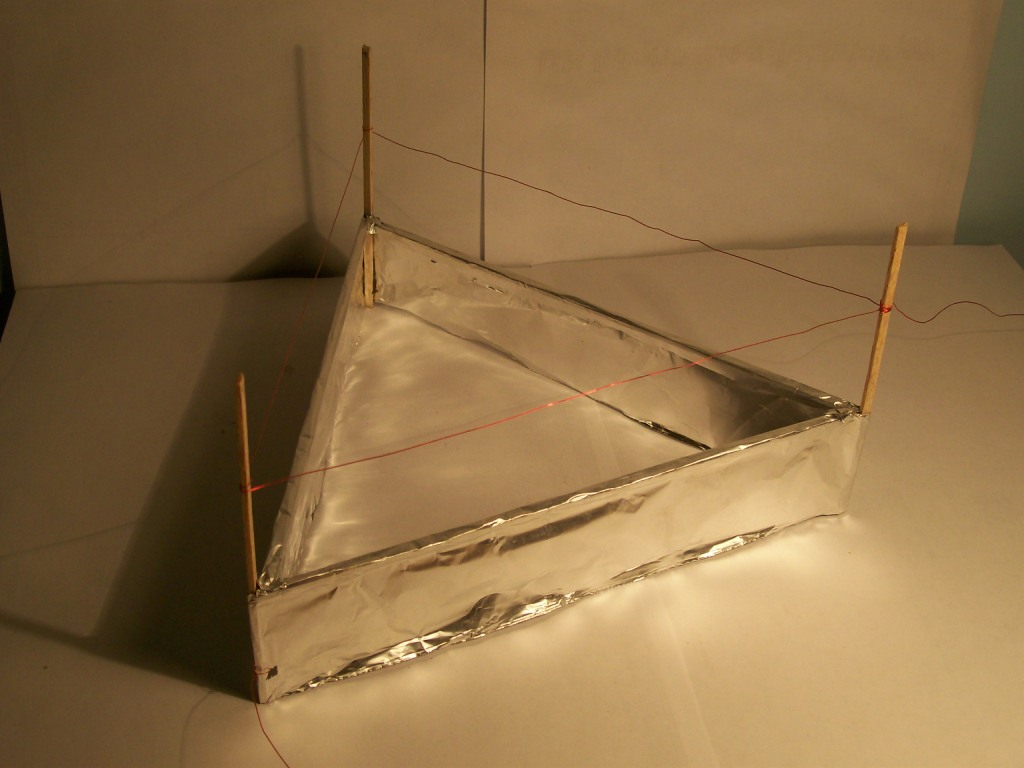
\includegraphics[scale=0.3]{img/photo1.jpg}
				\caption{Un lifter triangulaire}
			\end{figure}
		\end{frame}
	
		\begin{frame}{Problématique}
			Dans quelle mesure les paramètres géométriques du lifter influent-ils sur la charge utile transportable ?
			\begin{figure}
				\center
				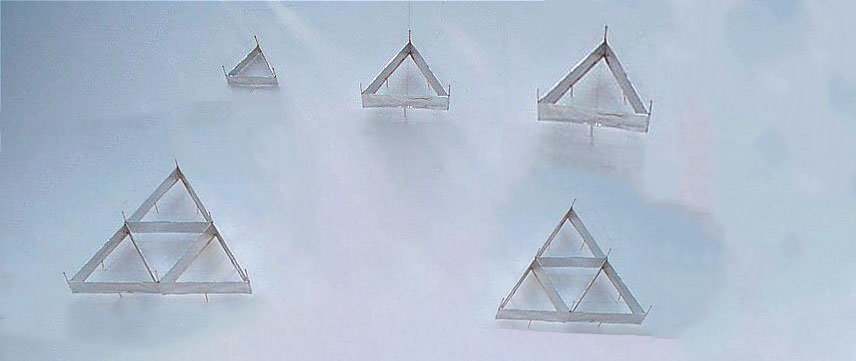
\includegraphics[scale=0.3]{img/lifters_p.jpg}
				\caption{Plusieurs lifters}
			\end{figure}
		\end{frame}

	\section{Paramétrage}

		\begin{frame}{Schéma}
			\begin{figure}
				\center
				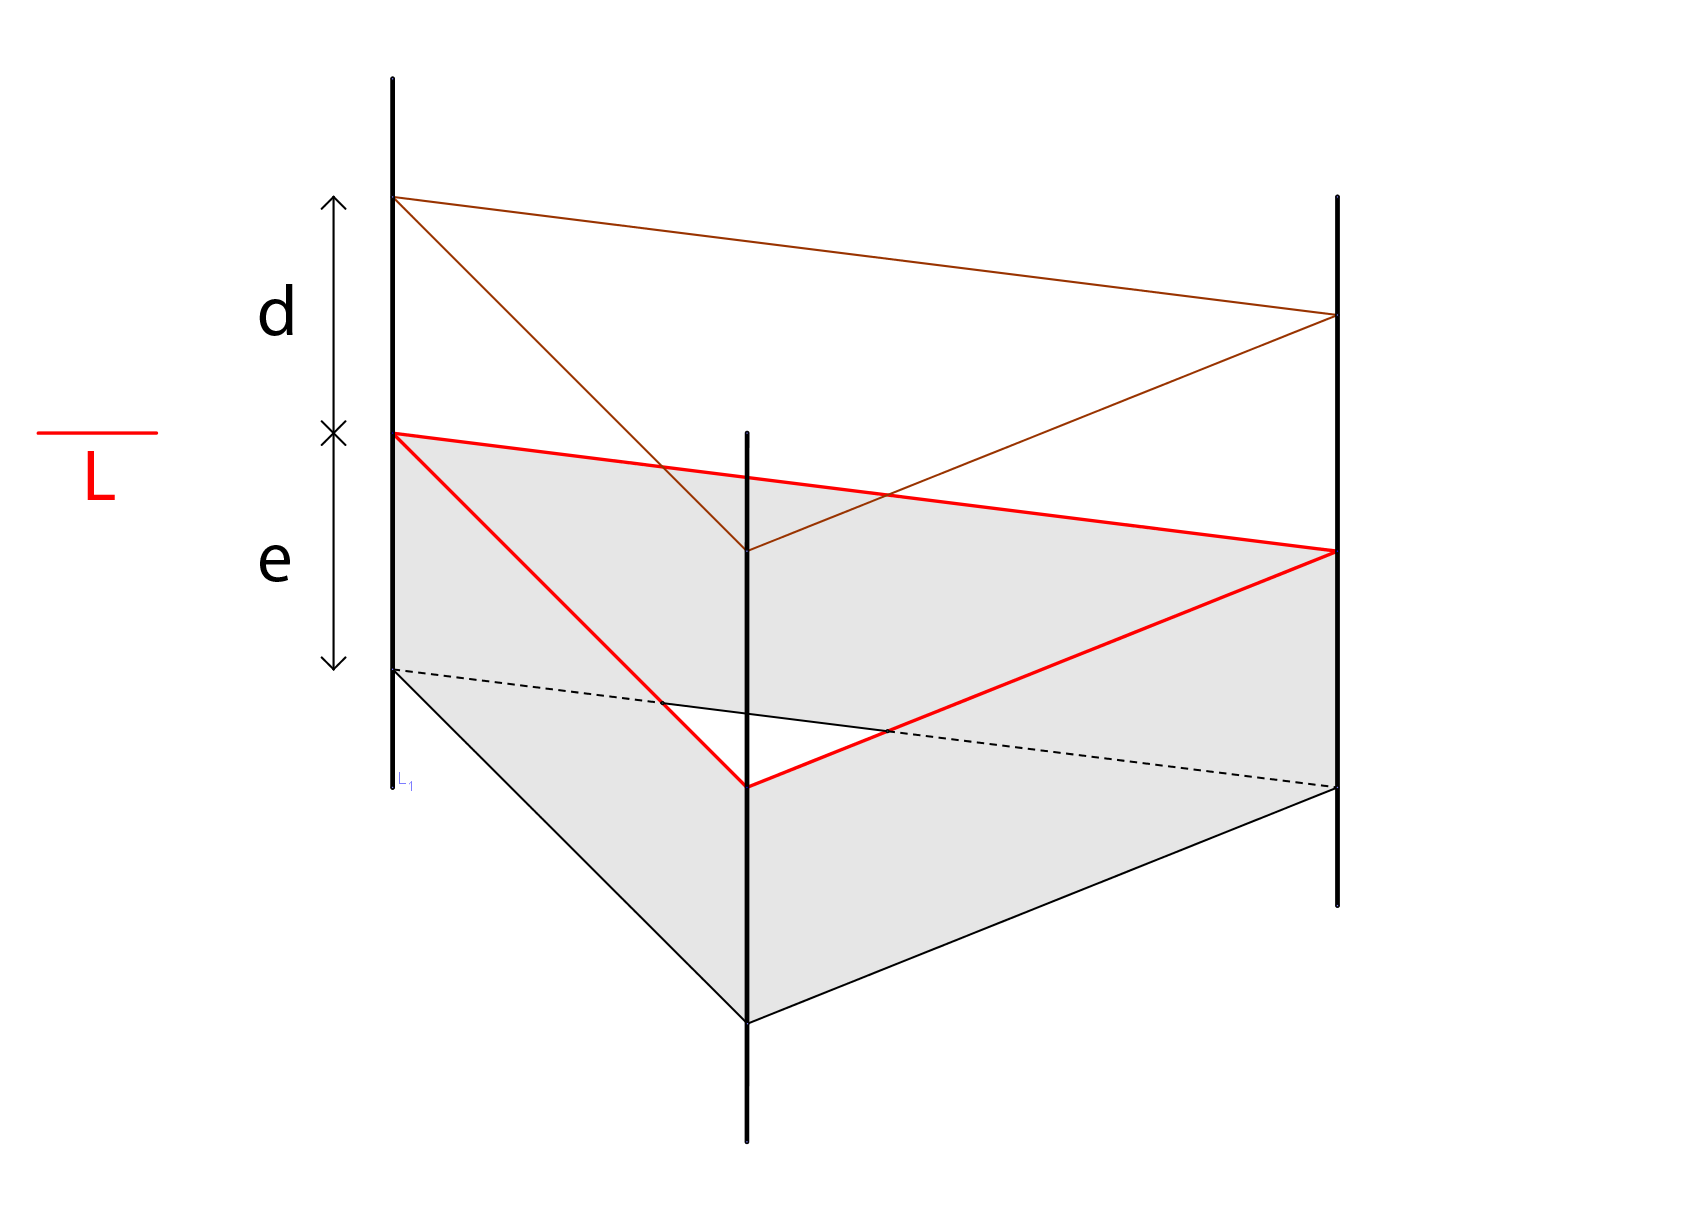
\includegraphics[scale=0.6]{img/lifter.png}
				\caption{Paramétrage du lifter}
			\end{figure}
		\end{frame}
	
		\begin{frame}{Paramétrage}
			\begin{itemize}
				\item Épaisseur de la bande $e$
				\item Rayon $r$
				\item Distance fil / bande $d$
				\item Périmètre $L$
				\item Polygone régulier $n$
			\end{itemize}
		\end{frame}
	
	\section{Expériences}
		\begin{frame}{Protocole général}
			\begin{itemize}
				\item Hypothèse : paramètres indépendants
				\item Variation d'\textbf{un paramètre}
				\item Plusieurs lifters
				\item Ajustement de la masse si nécessaire
			\end{itemize}
		\end{frame}
	
		\begin{frame}{Alimentation}
			\begin{itemize}
				\item THT : 20 kV
				\item Artisanale
			\end{itemize}
			\begin{figure}
				\center
				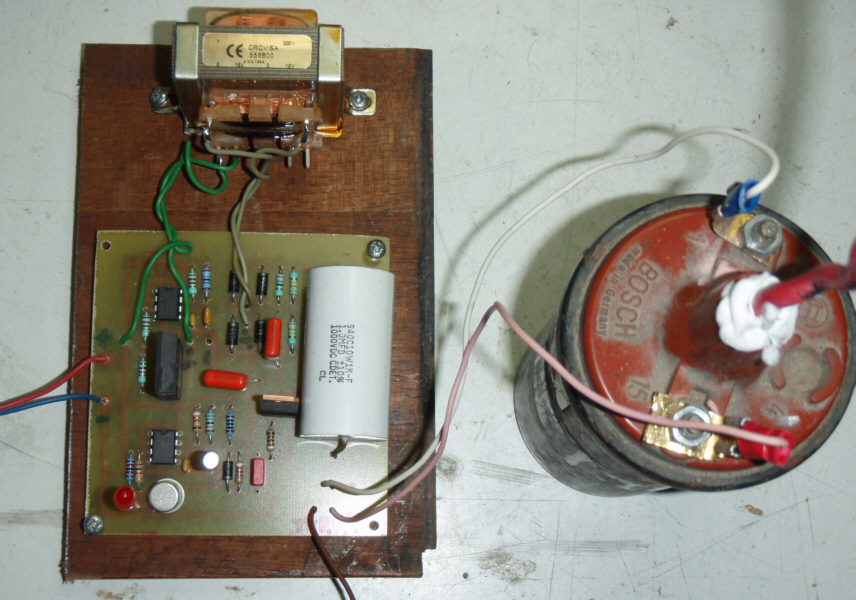
\includegraphics[scale=0.2]{img/alim.jpg}
				\caption{Alimentation THT}
			\end{figure}
		\end{frame}
	
		\begin{frame}{Montage}
			\begin{figure}
				\center
				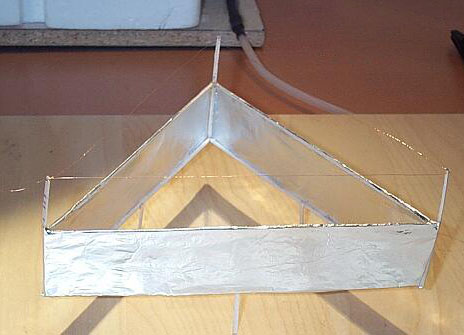
\includegraphics[scale=0.5]{img/photo2.jpg}
				\caption{Montage effectué}
			\end{figure}
		\end{frame}
	
		\begin{frame}{Ajustement de la masse}
			\begin{itemize}
				\item Masse caractéristique : 5 g
				\item Si $\Delta m > 0.01m_{max}$
				\item Boulettes d'aluminium
				\item Idem pour la charge utile
			\end{itemize}
		\end{frame}
	
		\begin{frame}{Épaisseur de la bande : protocole}
			\begin{itemize}
				\item 10 lifters triangulaires
				\item e : 3 à 7.5 cm
				\item Masses ajustées
			\end{itemize}
		\end{frame}
	
		\begin{frame}{Épaisseur de la bande : résultats}
			\begin{tikzpicture}
				\begin{axis}
				[
					width = \textwidth,
					height = \axisdefaultheight - 10,
					title = Charge utile $m_c$ en fonction de l'épaisseur $e$,
					xlabel = Épaisseur de la bande ($\pm 0.1$ cm),
					ylabel = Charge utile ($\pm 0.1$ g),
					ymin = 0,
					legend pos = outer north east,
				]
				\addplot[
					only marks,
					mark = *
				]
				table [
					x = e,
					y = mc,
					col sep = comma
				]
				{exps/epaisseur.csv};
				\end{axis}
			\end{tikzpicture}
		\end{frame}
	
		\begin{frame}{Épaisseur de la bande : conclusions}
			\begin{itemize}
				\item Affine entre 3 et 5.5 cm
				\item Constant au-delà
				\item Portée du champ magnétique ?
				\item \textbf{Meilleure configuration : e = 5.5 cm}
			\end{itemize}
		\end{frame}
	
		\begin{frame}{Rayon du fil : protocole}
			\begin{itemize}
				\item 4 lifters triangulaires
				\item r : 0.025 à 0.1 mm
				\item Masses non ajustées
			\end{itemize}
		\end{frame}
	
		\begin{frame}{Rayon du fil : résultats}
			\begin{tikzpicture}
				\begin{axis}
					[
						width = \textwidth,
						height = \axisdefaultheight - 10,
						title = Charge utile $m_c$ en fonction du rayon du fil $r$,
						xlabel = Rayon du fil ($\pm 0.1$ mm),
						ylabel = Charge utile ($\pm 0.1$ g),
						ymin = 0,
						legend pos = outer north east,
						xtick = data
					]
					\addplot[
						only marks,
						mark = *,
					]
					table [
						x = r,
						y = mc,
						col sep = comma
					]
					{exps/rayon.csv};
				\end{axis}
			\end{tikzpicture}
		\end{frame}
	
		\begin{frame}{Rayon du fil : conclusions}
			\begin{itemize}
				\item Quasi-constant
				\item \textbf{Meilleure configuration : r = 0.025 mm}
			\end{itemize}
		\end{frame}
	
	\begin{frame}{Distance fil/bande : protocole}
		\begin{itemize}
			\item 10 lifters triangulaires
			\item d : 0.5 à 5 cm
		\end{itemize}
	\end{frame}
	
	\begin{frame}{Distance fil/bande : résultats}
		\begin{tikzpicture}
			\begin{axis}
			[
				width = \textwidth,
				height = \axisdefaultheight - 10,
				title = Charge utile $m_c$ en fonction de la distance fil/bande $d$,
				xlabel = Distance fil/bande ($\pm 0.1$ cm),
				ylabel = Charge utile ($\pm 0.1$ g),
				ymin = 0,
				legend pos = outer north east,
			]
			\addplot[
				only marks,
				mark = *
			]
			table [
				x = d,
				y = mc,
				col sep = comma
			]
			{exps/distance.csv};
			\end{axis}
		\end{tikzpicture}
	\end{frame}
	
	\begin{frame}{Distance fil/bande : conclusions}
		\begin{itemize}
			\item Affine entre 0.5 et 2.0 cm
			\item Constant au-delà
			\item Portée du champ magnétique ?
			\item \textbf{Meilleure configuration : d = 2.0 cm}
		\end{itemize}
	\end{frame}

	\begin{frame}{Longueur : protocole}
		\begin{itemize}
			\item 7 lifters triangulaires
			\item L : 6 à 24 cm
			\item Masses non ajustées
		\end{itemize}
	\end{frame}

	\begin{frame}{Longueur : résultats}
		\begin{tikzpicture}
			\begin{axis}
			[
				width = \textwidth,
				height = \axisdefaultheight - 10,
				title = Charge utile $m_c$ en fonction de la longueur $L$,
				xlabel = Longueur L ($\pm 1$ cm),
				ylabel = Charge utile ($\pm 0.1$ g),
				ymin = 0,
				legend pos = outer north east,
				xtick = data
			]
			\addplot[
				only marks,
				mark = *
			]
			table [
				x = L,
				y = mc,
				col sep = comma
			]
			{exps/longueur.csv};
			\end{axis}
		\end{tikzpicture}
	\end{frame}

	\begin{frame}{Longueur : conclusions}
		\begin{itemize}
			\item Maximum entre 15 et 18 cm
			\item Plus grand $\longrightarrow$ plus massique
			\item \textbf{Meilleure configuration : L = 18 cm}
		\end{itemize}
	\end{frame}

	\begin{frame}{Géométrie générale : protocole}
		\begin{itemize}
			\item 4 lifters
			\item n : 3 à 6
			\item Mais seul le triangulaire a décollé
		\end{itemize}
	\end{frame}

	\begin{frame}{Géométrie générale : conclusion}
		\begin{itemize}
			\item Problème de fabrication / alimentation
		\end{itemize}
	
		\begin{figure}
			\center
			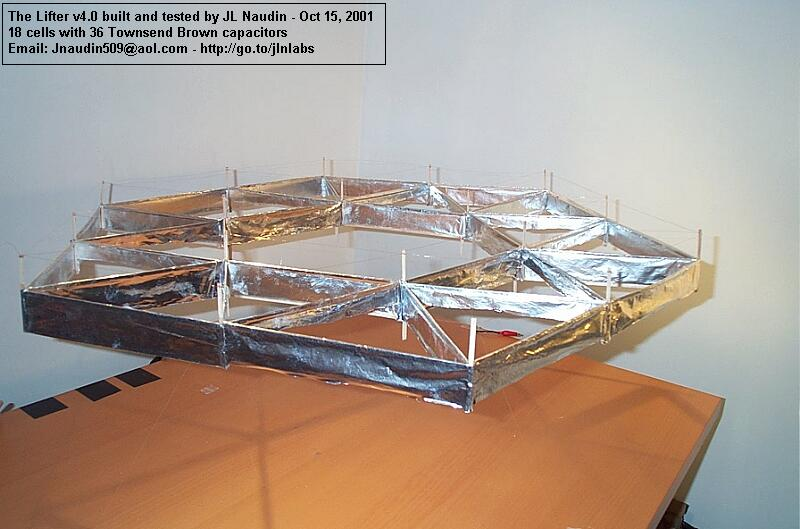
\includegraphics[scale=0.3]{img/lifter_naudin.jpg}
			\caption{Un lifter complexe par J.L. Naudin}
		\end{figure}
	\end{frame}

	\begin{frame}{Configuration retenue}
		\begin{itemize}
			\item Géométrie triangulaire
			\item e = 5.5 cm
			\item r = 0.025 mm
			\item d = 2.0 cm
			\item L = 18 cm
			\item $\Rightarrow m_c = 7.1$ g
		\end{itemize}
	\end{frame}

	\begin{frame}{Conclusions}
		\begin{itemize}
			\item Effet Biefeld-Brown est vérifié
			\item Configuration pas "optimale"
			\item Hypothèse : paramètres indépendants $\longrightarrow$ \textbf{fausse}
		\end{itemize}
	\end{frame}
\end{document}